\documentclass{standalone}
\usepackage{tikz}
\usetikzlibrary{decorations.pathmorphing,calc,3d}

\newsavebox{\videoin}
\savebox{\videoin}{%
  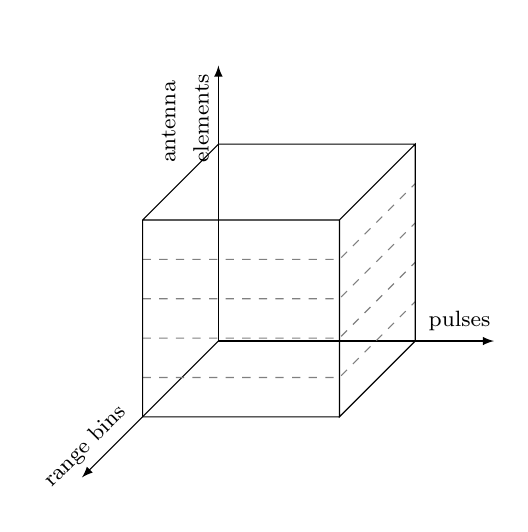
\begin{tikzpicture}[scale=.5,>=latex]
    \coordinate (o) at (0,0,0);
    \draw[->] (o) -- (0,0,9) node [very near end, above, sloped] {\footnotesize range bins};
    \draw[->] (o) -- (0,7,0) node [very near end, above, sloped, text width=1.6cm] {\footnotesize antenna elements};
    \draw[->] (o) -- (7,0,0) node [very near end, above, sloped] {\footnotesize pulses};

    \foreach \i in {1,...,4} {
      \draw[dashed,gray] (0,\i,5) -- (5,\i,5) -- (5,\i,0);
    }    
    
    \draw
    (0,5,0) -- (5,5,0)
    (0,5,0) -- (0,5,5) -- (0,0,5) -- (5,0,5)
    (0,5,5) -- (5,5,5)
    (5,0,0) -- (5,5,0) -- (5,5,5) -- (5,0,5) -- cycle;
  \end{tikzpicture}%
}

\newsavebox{\antenna}
\savebox{\antenna}{%
  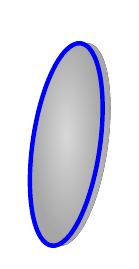
\begin{tikzpicture}[]
     \fill[inner color=gray!30,outer color=gray!70] (0,0,0) [x={(0,0,.4)}] circle (3 and 1.2);
     \fill[inner color=gray!30,outer color=gray!70] (-.1,0,0) [x={(0,0,.4)}] circle (3 and 1.2);
     \draw[ultra thick,blue](-.1,0,0) [x={(0,0,.4)}] circle (3 and 1.2);
  \end{tikzpicture}%
}

\begin{document}
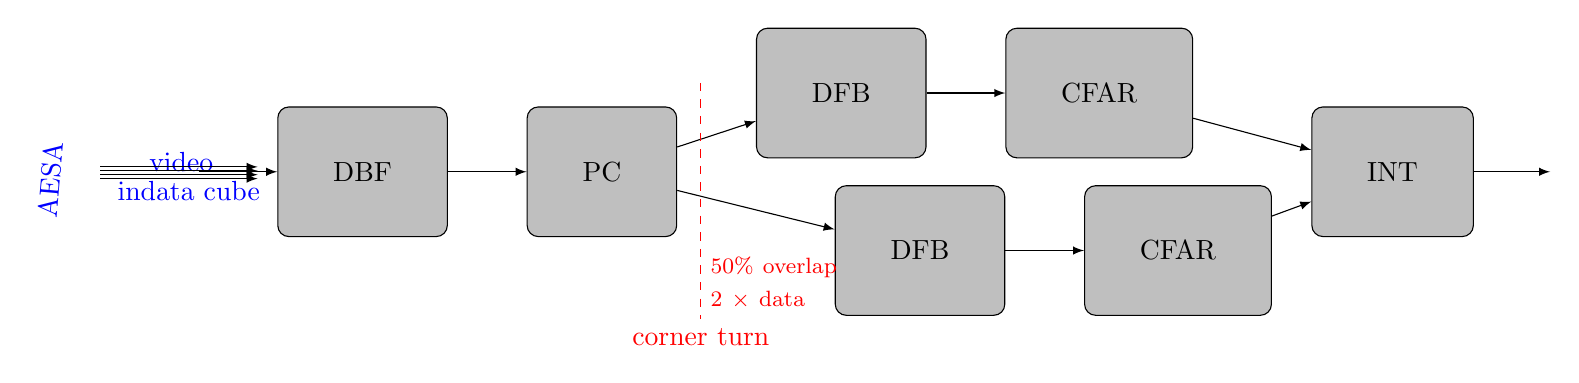
\begin{tikzpicture}[>=latex,
  right/.style={xshift=1cm,anchor=west},
  block/.style={draw, fill=gray!50, inner sep=20pt, rounded corners}]
  \node (antenna) {\usebox{\antenna}};
  \node[rotate=85,blue,xshift=-.1cm] at (antenna) {AESA};
  \node[anchor=west, xshift=1.5cm] (video) at (antenna.east) {\usebox{\videoin}};
  \node[blue,anchor=north] at (video) {indata cube};
  \node[blue,right] at (antenna.north east) {video};
  
  \foreach \i in {25,45,65,85} {
    \draw[->] ($(antenna.north east)!.\i!(antenna.south east)$)++(.5,0) --++(2,0);
  }

  \node[block,right] (dbf) at (video.east) {DBF}; 
  \node[block,right] (pc) at (dbf.east) {PC}; 
  \node[block,right,yshift=1cm] (dfb1) at (pc.east) {DFB}; 
  \node[block,right,yshift=-1cm,xshift=1cm] (dfb2) at (pc.east) {DFB};
  \node[block,right] (cfar1) at (dfb1.east) {CFAR};
  \node[block,right] (cfar2) at (dfb2.east) {CFAR};
  \node[block,right] (int) at ($(cfar1.east)!.5!(cfar2.east)$) {INT};

  \draw[->] (video) edge (dbf) (dbf) edge (pc) (pc) edge (dfb1) edge (dfb2) (dfb1) edge (cfar1) (dfb2) edge (cfar2) (cfar1) edge (int) (cfar2) edge (int) (int) edge++(2,0);
  \draw[dashed,red] ($(pc.north east)!.3!(dfb1.north west)$) -- ++(0,-3) node [anchor=north] {corner turn} node [anchor=south west,text width=1.8cm]{\footnotesize 50\% overlap 2 $\times$ data};
\end{tikzpicture}
\end{document}
